\documentclass[aps,prc,nofootinbib,showpacs,superscriptaddress,groupedaddress]{revtex4-1}
\usepackage{amsmath,amssymb,amsbsy,bm}
\usepackage{graphicx}
\usepackage{comment}
\usepackage{float}
%\usepackage{mathabx}
\usepackage[colorlinks=true,linkcolor=blue,citecolor=blue,urlcolor=blue]{hyperref}

\begin{document}

\title{Charge Conservation and Higher Moments of Charge Fluctuations}
\author{Scott Pratt}
\affiliation{Department of Physics and Astronomy and National Superconducting Cyclotron Laboratory\\
Michigan State University, East Lansing, MI 48824~~USA}
\author{Rachel Steinhorst}
\affiliation{Department of Physics and Astronomy\\
Michigan State University, East Lansing, MI 48824~~USA}
\date{\today}

\pacs{}

\begin{abstract}

\end{abstract}

\maketitle

\section{Introduction}\label{sec:intro}

The fluctuation of conserved charges is a standard means by which to investigate and classify phase transitions. At the critical point correlation lengths diverge, which results in peaks in charge fluctuations as one approaches the critical point. For systems with first-order phase transitions, fluctuations become infinite whenever one is in a region of phase separation, as the liquid and gas regions prefer to become infinite in extent when the surface energy is non-zero. The growth of fluctuations becomes increasingly dramatic as one considers progressively higher-order fluctuations. In a volume $V$, fluctuations of a charge $Q$ can be defined as
\begin{eqnarray}\label{eq:kappadef}
\mathcal{M}_N&\equiv&\frac{1}{V}\langle(Q-\overline{Q})^N\rangle=\frac{1}{V}\sum_n P_n(n-\overline{n})^N,
\end{eqnarray}
when particles have unit charge. The measure is increasingly sensitive to the tails of the multiplicity distribution, $P_n$, as $N$ increases. The free energy, $F\sim a_2(n-\overline{n})^2 + a_3(n-\overline{n})^3\cdots$, is minimized for $n=\overline{n}$, but the quadratic part vanishes at the critical point, $a_2\rightarrow 0$, which allow the fluctuations to grow and be dominated by higher-order terms. The shape of the tails of the distribution can be profoundly altered. 

The properties of the QCD  transition, deconfinement and the restoration of chiral symmetry, are not well understood at finite baryon density. There exists the possibility that this transition is a true phase transition, with a critical point at several times nuclear density and with a critical temperature close to the pion mass. If this is the case, it begs the question as to whether the conditions for phase separation or for critical phenomena can be reproduced in the laboratory. Heavy ion collisions at high energy, measured at the Relativistic Heavy Ion Collider (RHIC) or a the LHC, can produce mesoscopic regions a temperatures of a few hundred MeV, which is well above the expectations for a critical temperature, and densities of several times nuclear matter density. 

High-energy heavy ion collisions are characterized by strong explosive collective flow. Measurement is confined to the outgoing asymptotic momenta, but because of strong flow, correlations in coordinate space manifest themselves as correlations in relative momentum. Thus, measurements of correlations binned by relative momentum or charge fluctuations within some defined region of momentum space serve as surrogates for the corresponding observables in coordinate space. Indeed, measurements of charge and baryon number fluctuations have been performed at RHIC. By adjusting the beam energy of the colliding nuclei, experiments at RHIC have explored conditions at which novel phase phenomena might occur. Fluctuations of electric charge and baryon number have been especially popular. An initial scan of beam energies was rather inconclusive, but measurements with greatly improved statistics are currently being analyzed. 

In addition to the finite system size (event multiplicities might number in the thousands), the novel states of matter created in heavy-ion collisions persist for $\lesssim 10$ fm/$c$. This severely limits the degree to which phases can separate or to which critical fluctuations can grow. From the initial overlap of the colliding nuclei, until the mean time at which emitted particles experience their last collision, the collision lasts a few tens of fm/$c$. This limits the degree to which conserved charges can separate from one another. For example if a strange and an anti-strange quanta are produced together, their separation is limited by diffusion, and fluctuations of strangeness, or any other charge, requires that charges be given sufficient time to leave and enter the defining volume.

The goal of this paper is to gauge the degree to which charge-balance correlations affect higher-order correlations. In addition to making it difficult for phases to separate or for critical correlations to emerge, conservation also represents its own source of correlation, which needs to be understood as a potential sourcs of background before making firm arguments to have observed phenomena related to phase transitions. It is well known that charge-balance correlations are readily measurable at the two particle level, $N=2$ in Eq. (\ref{eq:kappadef}), and that they explain the bulk of the $N=2$ fluctuation measurement. However, their impact on $N=3,4$ fluctuations has not be investigated in great detail. For instance, the four-particle measure of correlation,
\begin{eqnarray}
C_4&=&\mathcal{M}_4-3\mathcal{M}_2^2,
\end{eqnarray}
which is based on cumulants, subtracts much of the contribution to the $\mathcal{M}_4$ coming from purely two-particle correlations. However, charge conservation can involve multiple particles, and the degree to which a cumulant-based measure, like the kurtosis, is affected by charge conservation is not fully understood. Relations based on a uniform acceptance probability and for a single type of charge were worked out in \cite{Savchuk:2019xfg}, which provide significant insight into how higher-order correlations are affected by charge conservation. The goal of this study is to extend such ideas to a more realistic picture, which takes into account the conservation of all three types of charge (baryon number, electric charge and strangeness) and applies a more realistic model of experimental acceptance and efficiency. The interplays of charge conservation with chemical equilibrium, decays and Bose statistics are all considered.

To understand the role of chemical equilibrium and decays, a model is presented which creates small volumes in which the net charge, $B,Q$ and $S$, is fixed at some value. Even if the net charges are all zero, charged particles exist but in combinations that conserve the net charge. Theoretical methods for exact calculation of the canonical ensemble and a method for Monte Carlo generation of statistically independent events are presented here. The method lends itself to including decays and accounting for experimental acceptance and efficiency. The physical picture of treating small volumes as independent patches was previously done for calculation of charge balance functions in \cite{Schlichting:2010qia,Schlichting:2010na}, and was also applied in \cite{Oliinychenko:2020cmr}. Following the terminology in \cite{Oliinychenko:2020cmr}, we refer to these sub-volumes as patches. The method presented here creates perfectly independent samplings, and can generate billions of such patches within a few hours. This enables highly accurate calculations of high moments with minimal numeric costs.

The next section reviews the definition of cumulants, skewness and kurtosis. Theoretical methods are presented in the next section. This includes a review of how one can exactly calculate canonical ensembles for multiple charges in a hadron gas and independently generate sets of particles for a given sub-volume, or patch.  Simplified expressions for a single type of charge with a fixed efficiency, which were derived and presented in \cite{Savchuk:2019xfg}, are also listed here as they provide a strong base from which to understand the behavior of more complicated treatments.

After a brief review of cumulants and the definitions of skewness and kurtosis in Sec. \ref{sec:cumulaants}, the method for exact solution of the canonical ensemble describing a multi-component, multi-charge hadron gas is presented in Sec. \ref{sec:theory}. These techniques extend those used for canonical ensembles used to study isospin fluctuations of a hadron gas \cite{}, nuclear fragmentation \cite{}, the level density of a Fermi gas, and the effect of restricting a quark-gluon plasma (QGP) to having fixed charge, including being in an overall color singlet \cite{}. Exact methods for calculating correlations up to fourth-order are presented. Unfortunately, to include realistic acceptance effects and complex decays, the exact expressions are no longer viable. However, as shown in Sec. \ref{sec:theoryMC}, the exact expressions show how sample events can be generated. An event, defined by a set of particles and momenta, are generated with perfect independence from one another, and perfectly reproduce the canonical expressions from Sec. \ref{sec:theoryexact}. Section \ref{sec:theorybosefermi} extends the previous sections to show how Bose correlations can be included. Section \ref{sec:uniformeff} considers the case of a single type of charge and a uniform efficiency, i.e. the probability of any particle being recorded is set to some fixed value. Much of this discussion repeats what is said in \cite{Savchuck:2019xfg}, and is included for completeness. This provides for a physical discussion of how charge conservation, volume fluctuations, chemical equilibrium, decays, clustering, and Bose corrections should affect higher moments.

The heart of this study is presented in Sec. \ref{sec:blastwave}. Here, the patches are assigned collective velocities consistent with the collective flow deduced from heavy-ion collisions. A canonical sampling of particles are generated from each patch, followed by a simulation of their decays. The particles were then overlaid onto the acceptance of the STAR detector at RHIC. Each patch is uncorrelated with any other patch, so moments can be calculated by averaging over the independent contributions from the patches. Results are displayed alongside results from the STAR Collaboration. The size and sign of the fluctuations of the net-proton distributions are consistent with observations, but the calculations of the net charge distributions differs qualitatively from STAR observations. A detailed discussion of the lessons derived from this study is presented in Sec. \ref{sec:summary}.

\section{Cumulants, Skewness and Kurtosis}

To keep the more manuscript self-contained, a brief review of cumulants and the definition of skewness and kurtosis is presented here.

Cumulants of a charge distribution are defined by 
\begin{eqnarray}
C_1&=\langle Q\rangle,\\
C_2&=\langle(Q-\overline{Q})^2\rangle,\\
C_3&=\langle(Q-\overline{Q})^3\rangle,\\
C_4&=\langle(Q-\overline{Q})^4\rangle-C_2^2,
\end{eqnarray}
where $Q$ is the net charge. Here, $Q$ might refer to baryon number, to strangeness, or to the electric charge measured in units of $e$.

Rather than showing the cumulants $C_n$, ratios are presented to help minimize trivial dependences on system size. The skewness, $S$, is a measure of the third moment,
\begin{eqnarray}
S&=\frac{C_4}{C_2^{3/2}}.
\end{eqnarray}
This definition has the advantage in being dimensionless, but it does not become independent of volume in the limit of large volumes. Thus, it is more common to consider the ratio
\begin{eqnarray}
S\sigma&=S\sqrt{C_2}=\frac{C_3}{C_2},
\end{eqnarray}
which becomes an intensive measure in the limit of larger volumes. The kurtosis is a measure of four-particle correlations,
\begin{eqnarray}
K&=\frac{C_4}{C_2^2},
\end{eqnarray}
but instead of $K$, one typically chooses
\begin{eqnarray}
K\sigma^2&=\frac{C_4}{C_2},
\end{eqnarray}
to find an intensive measure of the fluctuation, at least for large volumes. 

The measures $S\sigma$ and $K\sigma^2$ approach simple values in the limit that the distributions would be Poissonian. For Poissonian emission the observation of a charge in one region of momentum space is uncorrelated with the emission into any other space. Thus, particles are correlated only with themselves. If charges appear only in integral positive units, one can apply the usual expression for the Poissonian moments where the mean is $\eta$, 
\begin{eqnarray}
C_1&=\overline{n}=\eta\\
C_2&=\langle(n-\overline{n})^2\rangle=\eta,\\
C_3&=\langle(n-\overline{n})^3\rangle=\eta=C_1,\\
C_4&=\langle(n-\overline{n})^4\rangle-3C_2^2=\eta.
\end{eqnarray}
If there exist both positive and negative charges, the distribution of the net charge can be derived by convoluting the two distributions. Convoluting two Poissonians results in a Skellam distribution. If the mean number of positives is $\eta_+$ and the mean number of negatives is $\eta_-$, the distribution of net charge for a Skellam distribution, $Q=n_+-n_-$, yields the following cumulants
\begin{eqnarray}
C_1&=\eta_+-\eta_-,\\
C_2&=\eta_++\eta_-,\\
C_3&=\eta_+-\eta_-=C_1,\\
C_4&=\eta_++\eta_-=C_2.
\end{eqnarray}
Thus, if charges are produced in an uncorrelated fashion in increments of either $\pm 1$, the skewness and kurtosis become
\begin{eqnarray}
S\sigma&=\frac{C_3}{\sigma^2}=\frac{C_1}{\sigma^2},\\
K\sigma^2&=\frac{C_4}{\sigma^2}=1,
\end{eqnarray}
where $\sigma^2\equiv\langle(Q-\overline{Q})^2\rangle=\eta_++\eta_-$. It might have made more sense to consider $C_3/C_1$ rather than $S\sigma$, as that ratio would be unity in the limit that emission is uncorrelated. However, because experimental analyses have often concentrated on the two ratios above, higher order correlations in this paper will also be presented in terms of these ratios.

Moments depend on the efficiency $\alpha$ with which particles are measured. In the limit of vanishing efficiency all distributions of positives or of negatives tend to become Poissonian, and the distribution of the net charge will thus become a Skellam.  This can be understood by having the probability of observing a positive charge being $\alpha\rightarrow 0$ and the probability of observing two charges being proportional to $\alpha^2$ being negligible. This assumption would fall through if all positive charges were measured in pairs, i.e. multiple charges on each measured particle, but for final-state hadrons the charges are only $\pm 1$. As $\alpha\rightarrow 0$, the moments are dominated by the probability of observing either zero charges or a single charge, and the moments for counting particles of a given charge are
\begin{eqnarray}
\langle n^m\rangle&=\alpha,
\end{eqnarray}
for all $m>0$. It is then easy to see that $\langle (n-\overline{n})^m\rangle=\alpha$, which quickly leads to the result that as $K\sigma^2=C_3/C_1=1$.

If the net charge is fixed, a non-perfect efficiency is required to produce fluctuations. For fixed charge, the efficiency divides into two sets, the measured and non-measured. Each set fluctuates equally, but oppositely, relative to the mean. Thus, all the even moments of net charge will have an even reflection symmetry about an efficiency of $1/2$, and the odd moments will have an odd symmetry,
\begin{eqnarray}
\label{eq:alphasymm}
C_n(1/2+\delta\alpha)&=\left\{\begin{array}{rl}
C_n(1/2-\delta\alpha),&n=2,4,6\cdots\\
-C_n(1/2-\delta\alpha),&n=3,5,7\cdots~.\end{array}\right.
\end{eqnarray}

\section{Recursive Techniques for Generating Canonical Partition Functions}\label{sec:theoryexact}

For non-interacting particles the canonical partition function can be calculated exactly, or at least to the level that all partitions of $A\le A_{\rm max}$ hadrons are taken into account, with the exact solution being reached with $A_{\rm max}=\infty$. For our case, we conserve three quantities: the electric charge $Q$, the baryon number $B$ and the strangeness $S$. For states $i$ with energies $E_i$, the partition function,
\begin{eqnarray}
Z(Q,B,S)&=&\sum_{i,Q_i=Q,B_i=B,S_i=S}e^{-\beta E_i},
\end{eqnarray}
where $Q_i,B_i$ and $S_i$ are the discrete values of the conserved quantities for the state $i$, can be calculated recursively. The function $Z_A(Q,B,S)$ refers to the subset of states with $A$ hadrons,
\begin{eqnarray}
Z(Q,B,S)&=&\sum_{A\ge 0}Z_A(Q,B,S).
\end{eqnarray}
The recursive procedure begins with
\begin{eqnarray}
Z_{A=0}(0,0,0)&=&1,
\end{eqnarray}
is the canonical partition function of the vacuum. The contribution for a given $A$, $Z_A(Q,B,S)$, can be written as 
\begin{eqnarray}\label{eq:recurrence}
Z_A(Q,B,S)&=&=\frac{1}{A}\sum_h z_hZ_{A-1}(Q-q_h,B-b_h,S-s_h),
\end{eqnarray}
where $z_h$ is the single-particle partition function for hadron species $h$, which has charges $q_h,b_h$ and $s_h$. This was proved in \cite{Pratt:1999ht}, and can be understood by realizing that one can count all the ways to arrange $A$ hadrons with a given charge by considering all the ways to arrange one hadron multiplied by all the ways to arrange the remaining hadrons. To avoid double counting, a factor of $1/A$ is applied. For a fixed charge the probability to have $A$ hadrons is,
\begin{eqnarray}
P(A)&=&\frac{Z_A(Q,B,S)}{\sum_A Z_A(Q,B,S)}=\frac{Z_A(Q,B,S)}{Z(Q,B,S)}.
\end{eqnarray}
In practice, the sum over $A$ is cut off at some $A_{\rm max}$, but in our studies here that cutoff is made large enough that contributions to $Z$ for $A>A_{\rm max}$ are negligible. Thus, once builds the partition function from $A=0$ to $A_{\rm max}$ one has the partition function for all $Q,B,S$. 

Once the partition function is calculated one can also calculate the multiplicities and moments of observing specific species. For example, the multiplicity of species $h$ in a system with charge $Q,B,S$ is
\begin{eqnarray}
\langle N_h\rangle &= z_h\frac{Z(Q-q_h,B-b_h,S-s_h)}{Z(Q,B,S)}.
\end{eqnarray}
This also provides expressions for the various charges, e.g.,
\begin{eqnarray}
\langle Q\rangle &= \sum_h q_hz_h\frac{Z(Q-q_h,B-b_h,S-S_h)}{Z(Q,B,S)}.
\end{eqnarray}
Spectra can also be calculated
\begin{eqnarray}
\frac{dN_h}{d^3p}&=\frac{(2s_h+1)\Omega}{(2\pi\hbar)^3}e^{-E_h(p)}\frac{Z(Q-q_h,B-b_h,S-S_h)}{Z(Q,B,S)}.
\end{eqnarray}
Higher moments can also be extracted,
\begin{eqnarray}
\langle N_hN_{h'}\rangle &= \delta_{hh'}z_h\frac{Z(Q-q_h,B-b_h,S-s_h)}{Z(Q,B,S)}\\
&\hspace*{-30pt}+z_hz_{h'}\frac{Z(Q-q_h-q_{h'},B-b_h-b_{h'},S-s_h-s_{h'})}{Z(Q,B,S)}.
\end{eqnarray}
It is straightforward to extend this expression to the fluctuation of charges.

These expressions can also be extended to consider non-additive conservation laws. Net isospin conservation of a hadron gas was invoked in \cite{Cheng:2002jb}, i.e. restricting the states to being in an iso-singlet.  For quark-gluon states were restricted to being in both an iso-singlet and a color singlet in \cite{Pratt:2003jd}. For Bose corrections,
\begin{eqnarray}\label{eq:bose}
Z_A(B,Q,S)&=&\frac{1}{A}\sum_{h,n}z_{h,n}Z_{A-1}(Q-nq_h,B-nb_h,S-ns_h),\\
z_{h,n}&=&(2s+1)\sum_p e^{-nE_p/T}.
\end{eqnarray}
For the conditions of a hadron gas in high-energy heavy-ion collisions only pions are significantly affected by quantum degeneracy. 

For the case of a single kind of charge, one can see how the the recursive method above yields the same result as what one would expect by writing down the partition function for a system with $(A-Q)/2$ negative charges and $(A+Q)/2$ positive charges,
\begin{eqnarray}
\label{eq:singlecharge}
Z_{A,Q}=\left\{\begin{array}{rl}
\frac{z^A}{[(A-Q)/2]![(A+Q)/2]!},&A-Q~{\rm is~even},\\
0,&A-Q~{\rm is~odd}.\end{array}\right. ,
\end{eqnarray}
where $z$ is the partition function of a single charge. One can readily see that this is consistent with the recurrence relations,
\begin{eqnarray}
Z_{A,Q}&=&\frac{z}{A}\left\{Z_{A-1,Q-1}+Z_{A-1,Q+1}\right\}\\
\nonumber
&=&\frac{z}{A}\left\{\frac{z^{A-1}}{[(A-Q-2)/2]![(A+Q)/2]!}+\frac{z^{A-2}}{[(A-Q)/2]![(A+Q-2)/2]!}\right\}\\
\nonumber
&=&\frac{z}{A}\left\{\frac{z^{A-1}(A-Q)/2}{[(A-Q)/2]![(A+Q)/2]!}+\frac{z^{A-2}(A+Q)/2}{[(A-Q)/2]![(A+Q)/2]!}\right\}\\
&=&\frac{z^A}{[(A-Q)/2]![(A+Q)/2]!}.
\end{eqnarray}
This result is also equivalent to expectations based on setting reaction rates equal. If one assumes that pairs are created with some rate $\beta$, and that they are destroyed with some rate $\alpha N_+N_-$, where $N_+$ and $N_-$ are the number of positive and negative charges, $N_++N_-=A$. Setting the rates equal,
\begin{equation}\label{eq:ratesequal}
\alpha \frac{(A-Q)(A+Q)}{4}Z_{A,Q}=\beta Z_{A-2,Q}.
\end{equation}
One can not see that if one chooses $\beta/\alpha=z$ that Eq.s (\ref{eq:ratesequal}) and (\ref{eq:singlecharge}) are consistent.



Indeed, this result satisfies the recurrence relations above. If the net charge is zero, the result is even simpler,
\begin{eqnarray}
\label{eq:PAgivenQcanonical}
P(A|Q)&=&\frac{Z_{A,Q}}{\sum_A Z_{A,Q}},\\
\nonumber
P(A|Q=0)&=& \frac{z^A}{[(A/2)!]^2}\left\{\sum_{A={\rm even}} \frac{z^A}{[(A/2)!]^2}\right\}^{-1}.
\end{eqnarray}

Aside from the assumptions that $Q$ is fixed and there exists only one kind of charge, Eq.(\ref{eq:rateresult}) also requires that Bose and Fermi quantum statistical corrections are negligible, and that the charges come in unit charges. Despite these shortcomings, this picture is useful in that it allows one to see how multiplicities fluctuations are affected by charge conservation in a simple picture. 

One can also find $\omega_M$ by considering an equilibrated system. Here, we first consider an extremely simplified model of a system with only one conserved charge, and where the species all have charge of either $-1$ or $+1$. Again, the partition functions are labeled by the charge $Q$ and by the net number of hadrons $A$. Because particles have charges only of $\pm 1$, the partition function for $z=Z_{A=1,Q=1}=Z_{A=1,Q=-1}$ forms the basis of all other partition functions. From the methods of the previous section
\begin{eqnarray}
Z_{A,Q}&=\frac{z}{A}\left[Z_{A-1,Q-1}+Z_{A-1,Q+1}\right].
\end{eqnarray}
This relation rapidly reproduces the partition function for all $A$ and $Q$ for $A$ of the order of a few hundred.

\section{Generation of Uncorrelated Sample Events}\label{sec:theoryMC}

Complicated experimental acceptances are difficult to incorporate into expressions for the moments. It is then easiest to generate entire events via Monte Carlo, and filter the events through the acceptance. The Monte Carlo procedure involves choosing a hadron proportional the number of ways the system might have such hadron, i.e. a product of the partition function of the individual hadron multiplied by the partition function of the remainder. The procedure becomes:
\begin{enumerate}
\item Calculate and store the partition function, $Z_A(Q,B,S)$, up to some size $A\le A_{\rm max}$ for all $Q,B,S$ that might ultimately couple back to a given $A=A_{\rm max}$ for the given total values $Q,B,S$. 
\item For total charge $Q,B,S$, choose the number of hadrons $A$ proportional to $Z_A(Q,B,S)/Z_A(Q,B,S)$.
\item Choose a hadron $h$ proportional to the probability $z_hZ_{A-1}(Q-q_h,B-b_h,S-s_h)/Z_A(Q,B,S)$. If Bose degeneracy is to be taken into account this procedure is slight modified as described in Sec. \ref{sec:bose}.
\item Choose the momentum proportional to the thermal weight $e^{-E_p/T}$.
\item Repeat (3,4) but with $A,Q,B,S$ being replaced by $A-1,Q-q_h,B-b-h,S-s_h$. The procedure is finished when $A=0$.
\end{enumerate}
Bose effects for pions can be included by altering the second and third steps above. In addition to choosing a hadron, one might also consider adding a $2-$pion, $3-$pion or $n-$pion state. Simply treat the $n-$pion state as if it were a resonance with charges $nq_h,nq_b,nq_s$, but with a partition function $z_{h,n}$ described above. If one chooses to make such a ``particle'', the $n$ identical particles are are given the same momentum and spin projection, using a Boltzmann distribution with a temperature $T/n$. To be more realistic the momenta should be smeared by some momenta $\approx\hbar/R$, where $R$ is a characteristic size of the system. If Fermi effects were to be included, one could calculate the partition function by adding a factor $(-1)^{n-1}$ to each term in the sum described in Eq. (\ref{eq:bose}). However, because some of the weights are negative, Monte Carlo procedures can become problematic. Fortunately, for the systems considered here are extremely hot, and degeneracy of fermions is negligible.

Storing the partition function can require substantial memory for larger $A_{\rm max}$ because the indices $Q,B$ and $S$ must also vary over a range of order $\pm A_{\rm max}$, so memory usage roughly scales with $A_{\rm max}^4$. Because one is usually interested in calculations with total charge near zero, one can ignore partition functions for charges that cannot couple back to the fixed overall charge at $A_{\rm max}$. Once $A$ exceeds $A_{\rm max}/2$, the calculations here cutoff values of $Q,B$ and $S$ that could not ultimately affect the $Q=B=S=0$ partition function for $A=A_{\rm max}$. Even with this savings, partition functions with $A_{\rm max}=250$ could require approximately 13 GB of memory, and need on the order of 10 minutes to calculate on a single processor. For $A_{\rm max}=125$, less than a GB of memory was needed and partition functions could be calculated in less than a minute. For hadron gases at temperatures of 150 MeV, $A_{\rm max}=250$ was readily sufficient for patch volumes $\lesssim 700$ fm$^3$. If multiple patch volumes are to be explored for the same temperature, computational time can also be saved by realizing that the partition functions scale as $\Omega^A$. Thus, if one performs a calculation for some initial volume $\Omega_0$, scaling can provide results for new volumes with minimal computation.

Once the partition function is calculated, event generation is remarkably fast. The time to generate an even scales linearly with the volume, or equivalently, linear with the average number of particles generated. Running sufficient events to generate a million individual particles can be accomplished within a few seconds on a single CPU. Unlike Metropolis methods where events are modified by considering small changes to existing events, such as in \cite{}, each event in this is independent as long as the random numbers are without correlation.

\section{Bose and Fermi Statistics}\label{sec:theorybosefermi}

Including Bose and Fermi statistics in calculating the partition functions is straight-forward, and was shown in \cite{}. The method is related to that used for calculating the effects of multi-boson interference for pion interferometry. In a fixed volume the partition function can be first treated as the usual procedure of accounting for $n$ identical particles being in different single-particle states. This includes the $1/n!$ term to account for the fact that particles are indistinguishable, i.e. the Gibbs paradox. If $m_\ell$ indestinguishable particles are in the same single-particle state $\ell$, one must correct the weight by a factor of $m_\ell!$ for each level, which can also be thought of as the analog of the symmetrized relative wave function with all the momenta being equal. For fermions, the weight becomes $(-1)^{\ell-1}m_\ell$. As demonstrated in \cite{}, the recurrence relation to the partition function then becomes
\begin{eqnarray}\label{eq:Zbf}
Z_{A}(Q,B,S)&=\frac{1}{A}\sum_h \sum_n Z_{A-n}(Q-nq_h,B-nb_h,Q-nq_h)z_{h,n}(\pm 1)^{n-1},
\end{eqnarray}
where $z_{h,n}$ is the partition function for $n$ particles in any level, 
\begin{eqnarray}
z_{h,n}&=\sum_\ell e^{-n\beta(\epsilon_\ell-\mu_iq_i)}.
\end{eqnarray}
The $\pm 1$ refers to bosons or fermions. For hadron gases in the high temperature environments of relativistic heavy ion collisions, only pions have a non-negligible correction from quantum degeneracy. The correction for order $n$ for any level $\ell$ is of the order $e^{-\beta(\epsilon_\ell-\mu_iq_i)}$ lower than the previous term. This factor is largest for zero momentum, and for pions becomes $e^{-\beta(m-\mu)}$. The chemical potential is $\mu_Q q_i$ if the pions are chemically equilibrated, but if the system is not chemically equilibrated $\mu$ is adjusted to fit the average pion density. For the zero-momentum level at a temperature of 150 MeV, the factor is $e^{-m/T}\approx 0.4$, and as the system cools probably falls slightly \cite{gong}. For a more characteristic thermal momentum the factor is $\approx 0.1$. For heavier particles the factor is always small. For example, for a zero-temperature $\rho$ meson the factor is a fraction of a percent.

Given that symmetrization is only being applied to pions, which are bosons, one can incorporate these corrections into the Monte Carlo procedure outlined in Sec. \ref{sec:theoryMC}. For fermions this might be problematic because of the negative weights coming from the $(-1)^(n-1)$ factors in Eq (\ref{eq:Zbf}). Here, the algorithm is adjusted by treating each value of $n$ as being a different species, with charges $nq_h$ and with the partition function calculated with a reduced temperature $T\rightarrow T/n$. If one picks such a species in step 3 of the algorithm, $n$ pions are generated, all with the same momentum. For a finite system, the pions would have a small relative momentum or order the inverse system size.

It is well known that bosonic effects can broaden multiplicity distributions \cite{negativebinomial}, making them super-Poissonian. One of the goals of this study is to discern how bosonic statistics alter the kurtosis or skewness. 

\section{Models with Uniform Efficiency and Fixed Charge}\label{sec:uniformeff}

Even for a volume of fixed charge, finite efficiency and acceptance leads to non-zero fluctuations. The degree to which these fluctuations affect the skewness and kurtosis was worked out in \cite{Savchuk:2019xfg} for emission of a fixed charge where the probability of any charge being observed was a constant $\alpha$. If $\alpha$ were zero or unity, there would be no fluctuations, and because the charge on those particles that are not observed must fluctuate exactly opposite to the charge that is observed, the even moments must be symmetric about $\alpha=1/2$, and the odd moments must be anti-symmetric. One of the most important results of \cite{Savchuk:2019xfg} is that for fixed $Q$ and $\alpha$ the ratios cumulants depends only on $\alpha$ and the variance and mean of the underlying multiplicity distribution. Even though $Q$ is fixed, the net number of charged particles $M$ can fluctuate. 

From \cite{Savchuk:2019xfg}, the probability that $N$ charged particles with total charge $Q$ will result in a measured charge $q$ due to a uniform efficiency $\alpha$ is the convolution of two binomial distributions
\begin{eqnarray}
P(q|M,Q)&=&\sum_{n_+=0}^{(M+Q)/2}\sum_{n_-=0}^{(N-Q)/2}\frac{[(M+Q)/2]![(M-Q)/2]!}{[(M+Q)/2-n_+]![(M-Q)/2-n_-]!n_+!n_-!}
\alpha^{n_++n_-}(1-\alpha)^{M-n_+-n_-}.
\end{eqnarray}
After some tedious algebra, one can find the cumulants for fixed multiplicity,
\begin{eqnarray}
C'_1&=&\overline{q}=\alpha Q,\\
\nonumber
C'_2&=&\langle (q-\overline{q})^2\rangle_M = \alpha(1-\alpha)M,\\
\nonumber
C'_3&=&\langle (q-\overline{q})^3\rangle_M = \alpha(1-\alpha)(1-2\alpha)Q,\\
\nonumber
C'_4&=&\langle(q-\overline{q})^4\rangle_M -3\langle(q-\overline{q})^2\rangle_M^2\\
\nonumber
&=&\alpha(1-\alpha)-6\alpha^2(1-\alpha)^2M.
\end{eqnarray}
Here, the primes emphasize that the averages $\langle\cdots\rangle_M$. denote that they consider only those events with fixed base multiplicities $M$. The even moments are all linear in $M$, while the odd moments are linear in $Q$. It might appear that due to the linearity one might replace $M$ with $\langle M\rangle$ for a fluctuating base multiplicity, but the second term in the fourth cumulant
\begin{eqnarray}
-3\sum_M P(M) \langle(q-\overline{q})^2\rangle_M^2 &\ne&
-3\langle(q-\bar)^2\rangle^2.
\end{eqnarray}
Instead,
\begin{eqnarray}
\langle(q-\bar)^2\rangle^2&=&\alpha^2(1-\alpha)^2\overline{M}^2.
\end{eqnarray}
This provides a contribution to $C_4$ and the cumulants and their ratios become \cite{Savchuk:2019xfg},
\begin{eqnarray}
\label{eq:savchuck}
C_1&=&\alpha Q,\\
\nonumber
C_2&=&\alpha(1-\alpha)\overline{M},\\
\nonumber
C_3&=&\alpha(1-\alpha)(1-2\alpha)Q,\\
\nonumber
C_4&=&\alpha(1-\alpha)-6\alpha^2(1-\alpha)^2\overline{M}\\
\nonumber
&&+3^2\alpha(1-\alpha)^2\langle(M-\overline{M})^2\rangle,\\
\nonumber
\frac{C_2}{C_1}&=&(1-\alpha)\frac{\overline{M}}{Q},\\
\nonumber
\frac{C_3}{C_1}&=&(1-\alpha)(1-2\alpha),\\
\nonumber
\frac{C_3}{C_2}&=&(1-2\alpha)\frac{Q}{\overline{M}},\\
\nonumber
\frac{C_4}{C_2}&=&1+3\alpha(1-\alpha)(\omega_M-2),\\
\nonumber
\omega_M&\equiv&\frac{\langle(M-\overline{M})^2\rangle}{\overline{M}}.
\end{eqnarray}
The relative variance of the multiplicity of the base distribution, $\omega_M$, is unity for a Poissonian distribution. In that case $C_3/C_1$ and $C_4/C_2$ fall below unity for non-zero $\alpha$. The only assumptions for this relation are that the charge is fixed and that the efficiency is uniform. This is important as it implies that if one understands the efficiency and the second moment of the base multiplicity distribution, one can construct a baseline of cumulant ratios, and attribute any deviation from the baseline as due to fluctuations in $Q$, which is precisely the goal.

A reasonable value of $\alpha$ can be taken from balance function analyses. If a charge is observed, there should be a balancing charge emitted nearby, and detected with probability $\alpha$. This should correspond to the integrated strength of the charge balance function, which for electric charge is in the neighborhood of 0.4. Of course, $\alpha$ is not a constant. If a charge is observed in the center of the detector, its balancing charge has a better chance of being observed than for one observed near the periphery of the acceptance. Nonetheless, for the purposes of roughly setting expectations, this suggests that $C_4/C_2$ can be significantly differ from unity. 

Equation (\ref{eq:savchuck}) is crucial as it demonstrates that the fourth moment of the charge distribution is determined completely by the efficiency and the relative variance of the base multiplicity distribution, if the total base charge $Q$ is fixed. Next, we consider how various effects, aside from fluctuating the base charge $Q$, might push $\omega_M$ to be either super-Poissonian, $\omega_M>1$ or sub-Possonian. We discuss the effects of volume fluctuations, equilibrated charge distributions, decays and Bose condensation.

\subsection{Volume Fluctuations}\label{sec:volumefluc}

Heavy ion experiments measure collisions spanning a range of impact parameters. Even for a fixed impact parameter, energy deposition might significantly vary depending on how many nucleons actually collided or how many jets were produced. If more energy is deposited into a fixed volume, it might expand further before it hadronizes, resulting in larger final volumes. Experimental analyses attempt to minimize these fluctuations by constraining a given fluctuation measurement to a specific centrality bin, where ``centrality'' might be defined by multiplicity, transverse energy, or energy deposition in a forward calorimeter. To reduce auto-correlation centrality measurements are usually constrained to particles other than those used to construct the moments. Nonetheless, it is inevitable that a range of initial conditions is explored within any centrality bin, and one might thus expect the base multiplicity distribution to broaden. If the patch volumes are fixed at some constant value, volume fluctuations can be thought of as a fluctuation in the number of patches. 

It is tempting to expect that the ratio of cumulants would be independent of the number of patches, and thus impervious to volume fluctuations. Independently, each cumulant, $C_n$, scales linearly with the number of patches because there are no cross correlations between patches. Thus,
if $P_p(N)$ is the probability of having $N$ patches, and if $c_n$ is the cumulant for a single patch, the cumulant for the overall system is
\begin{eqnarray}
\label{eq:patchprob}
C_n&=&\sum_NP_p(N) Nc_n,
\end{eqnarray}
and the ratio of cumulants is 
\begin{eqnarray}
\frac{C_n}{C_m}&=&\frac{\sum_NP_p(N)Nc_n}{\sum_MP_p(M)Mc_m}\\
\nonumber
&=&\frac{c_n}{c_m}.
\end{eqnarray}
Thus, the ratio of cumulants is independent of the number of patches, and thus independent of the overall volume, but the ratio can still depend on the volume of an individual patch.

Unfortunately, although the ratios of cumulants are independent of the overall volume, they are not impervious to fluctuations of the overall volume, or equivalently, to fluctuations of the number of patches \cite{volumefluc}. To illustrate this, one can consider a system with a distribution $P_p(N)$  as in Eq. (\ref{eq:patchprob}), where the average number of patches is $\overline{N}$. For $n>1$ the cumulants are expressed in terms of $\delta Q=Q-\overline{Q}$. Because $\overline{Q}$ varies with the number of patches we rewrite it as
\begin{eqnarray}
\delta Q&=&\delta Q_N+\delta N\overline{Q}_1,\\
\delta Q_N&\equiv&Q-N\overline{Q}_1,
\end{eqnarray}
where $\overline{Q}_1=c_1$ is the average charge in a single patch. Here $\delta Q_N$ is the fluctuation of the charge for a specific number $N$ of patches, and $\delta N=N-\overline{N}$. Inserting these definitions into the expressions for the cumulants,
\begin{eqnarray}\label{eq:volfluc}
C_1&=&\kappa_1c_1,\\
\nonumber
C_2&=&\sum_NP_p(N) \langle(\delta Q_N+\delta N\overline{Q}_1)^2\rangle=\kappa_1c_2+\kappa_2c_1^2,\\
\nonumber
C_3&=&\sum_NP_p(N) \langle(\delta Q_N+\delta N\overline{Q}_1)^3\rangle=\kappa_1c_3+\kappa_3c_1^3,\\
\nonumber
C_4&=&\sum_NP_p(N) \langle(\delta Q_N+\delta N\overline{Q}_1)^4\rangle-3C_2^2\\
\nonumber
&=&\kappa_1c_4+3\kappa_2c_2^2+6\kappa_3c_2c_1^2+c\kappa_4c_1^4,
\end{eqnarray}
where $\kappa_n$ are the cumulants of $P_p(N)$,
\begin{eqnarray}\label{eq:kappadef}
\kappa_1&=&\sum_N NP_p(N)=\overline{N},\\
\nonumber
\kappa_2&=&\sum_N (N-\overline{N})^2P_p(N),\\
\nonumber
\kappa_3&=&\sum_N (N-\overline{N})^3P_p(N),\\
\nonumber
\kappa_4&=&\sum_N (N-\overline{N})^4P_p(N)-3\kappa_2^2.\\
\end{eqnarray}
If the number of patches are fixed, i.e. the overall volume does not fluctuate, then $\kappa_{n>1}=0$ and each cumulant satisfies $C_n=\overline{N} c_n$. The ratio of cumulants then cancels the factor $\overline{N}$. 
Once the volume fluctuates the ratios of cumulants of the charge distribution depends on the ratio of cumulants of $P_p(N)$. Methods have been constructed to eliminate the dependence volume fluctuations \cite{Begun:2014boa,Gazdzicki:2013ana,Gorenstein:2011vq,Sangaline:2015bma}. These methods are built on the assumption that the observable used to identify the volume is correlated to the fluctuating charge only through the fact that they both scale with the volume. If the phase space used for the centrality measure is clearly distinct of the phase space over which charge is measured, this should be a good approximation. 

It should be noted that the expressions in Eq.s (\ref{eq:volfluc}) and (\ref{eq:kappadef}) are built on the assumption that the average charge scales linearly with the number of patches. This differs from the assumptions going into Eq. (\ref{eq:savchuck}), where it was assumed that charge was fixed within the overall volume. If the total charge in the volume is absolutely fixed despite fluctuations in the number of patches, then volume fluctuations affect the answer in that the relative variance of the multiplicity distribution, $\omega_M$, is increased by volume fluctuations as described in Eq. (\ref{eq:savchuck}).

\subsection{Chemically Equilibrated Distribution}

One can also calculate $\omega_M$ for an equilibrated system of a single type of charge, where the measurement directly samples the equilibrated distribution. This ignores decays, which in later stages proceed without the regeneration needed to maintain equilibrium. The results of the equilibrated canonical ensemble in Eq. (\ref{eq:PAgivenQcanonical}) can be used to find $\omega_M$, and thus generate the moments using Eq. (\ref{eq:savchuck}). For large average multiplicities, $\overline{M}$, the value of $\omega_M$ approaches unity, the Poissonian limit. For small $\overline{M}$ it approaches two. This is expected, because for a fixed charge, you can only add particles pair-wise. In fact, as will be shown in the next section, if one generated a Poissonian number of pairs, the relative variance would be $\omega_M=2$ for all multiplicities. With $\omega_M$ near unity for any system of significant size the values of $C_4/C_2$ and $C_3/C_1$ stay below unity as shown in Fig. \ref{fig:savchuck}. 

\begin{figure}
\centerline{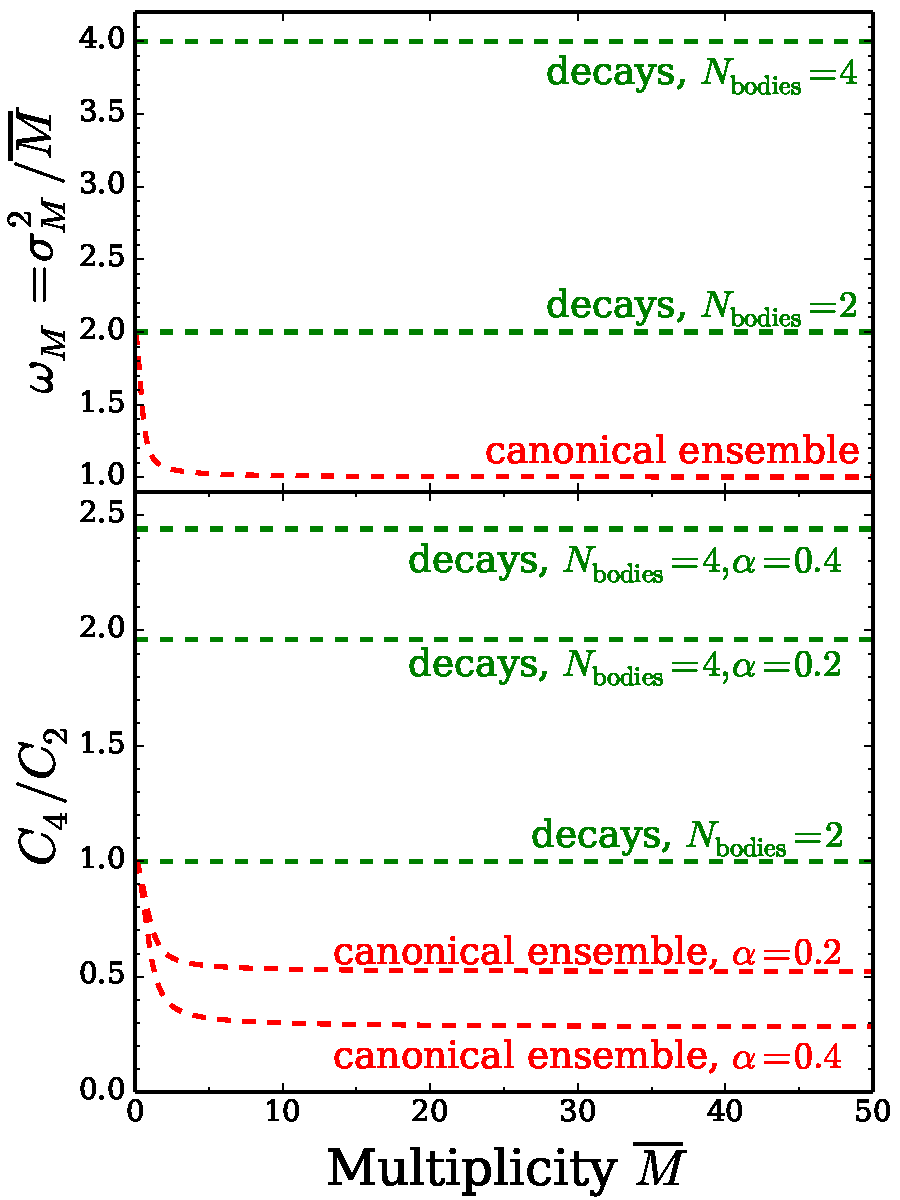
\includegraphics[width=0.5\textwidth]{figs/savchuck}}
\caption{\label{fig:savchuck}
The relative variance of the charged multiplicity distribution is shown for three cases in the upper panel for a system carrying only a single type of unit $\pm$unit charge. For a neutral equilibrated system $\omega$ approaches the Poissonian limit for higher mean multiplicities, $\overline{M}$. This contrasts to a system where one has a Poissonian distribution of neutral particles which all decay into pairs. In this case $\omega=2$ and if the number of charged particles coming from the decay, $N_{\rm bodies}$, of the neutral decay were $n$, one would have $\omega=n$. Using Eq. (\ref{eq:savchuck}) from \cite{savchuck} the ratio $C_4/C_2$ is plotted for the cases above for different fixed efficiencies $\alpha$. For $\omega<2$, $C_4/C_2$ falls below unity, and for $\omega>2$ the ratio exceeds unity. The difference from unity is strongest for $\alpha$ near $1/2$, and the result is symmetric for reflecting $\alpha$ about $1/2$. For $\alpha$ approaching zero or unity $C_4/C_2\rightarrow 1$.}
\end{figure}

\subsection{Decays}

In addition to the results from the canonical ensemble, a system of uncorrelated neutral particles that decays to charged particles is also presented to illustrate the difference in how charge conservation manifests itself in fluctuation observables depending on whether the charges arise directly from an equilibrated system, or whether they arise from the decays of uncorrelated neutral particles. Here, the multiplicity of the uncorrelated neutral particles is assumed to be Poissonian. If each neutral particle decays into $N_{\rm bodies}$ charged particles, where the charges are $\pm 1$, the charged particle multiplicity distributions become 
\begin{eqnarray}
\langle M_{\rm ch}\rangle&=&N_{\rm bodies}\overline{M}_0,\\
\nonumber
\langle(M_{\rm ch}-\overline{M}_{\rm ch})^2\rangle&=&N_{\rm bodies}\langle(M_0-\overline{M}_0)^2\rangle,\\
\nonumber
\omega_M&=&\frac{\langle(M_{\rm ch}-\overline{M}_{\rm ch})^2\rangle}{\overline{M}_{\rm ch}}\\
\nonumber
&=&N_{\rm bodies}\frac{\langle(M_0-\overline{M}_0)^2\rangle}{\overline{M}_0}.
\end{eqnarray}
Fig. \ref{fig:savchuck} illustrates how this picture affects $C_4/C_2$. In this case, because $\omega$ depends only on $N_{\rm bodies}$ and does not change with multiplicity or system size, the cumulants are also independent of multiplicity. For $N_{\rm bodies}=2$ the cumulant ratios does not even depend on the efficiency. For $N_{\rm bodies}>2$ the ratio $C_4/C_2$ exceeds unity, so if charge creation proceeded through the creation and decay of neutral clusters it would be easy to generate large values of $C_4/C_2$. This has been discussed at length in \cite{Bzdak:2018uhv}.

In an equilibrated system decays and recombination have equal rates. However, as the system decouples recombination stops and decays proceed until only stable hadrons remain. Very few decays proceed via more than on charged pair. During the hadronic phase the number of charged particles nearly doubles due to these decays. Thus, if the systems do equilibrate, then decay after chemical freeze-out, one would expect the ratio $C_4/C_2$ to lie somewhere between the value for the canonical ensemble in Fig. \ref{fig:savchuck} and the value for pure decays with $N_{\rm bodies}=2$. STAR's experimental results for net proton fluctuations indeed satisfy this expectation, but their measured $C_4/C_2$ for net charge fluctuations well exceed unity. This discrepancy could be due to volume fluctuations or the decay of larger clusters, or perhaps some shortcoming in this overly simple picture, e.g. the neglect of other conservation laws or Bose condensation. 

\subsection{Bose correlations}

It has long been understood that Bose correlations induce super-Poissonian fluctuations. Here, we illustrate how Bose effects combine with charge conservation to determine $C_4/C_2$. Partition functions for a gas of positive and negative pions, $m_\pi=139.57$ MeV/$c^2$, were considered to be kinetically equilibrated but with a chemical potential enforcing a fixed average density. If a gas is created at chemical equilibrium one expects $\mu=0$, but if it cools while maintaining a fixed number of pions, and if the pion number is fed by decays, a non-zero value of $\mu$ is required. At decoupling one expects kinetic temperatures to fall near 100 MeV and the pion chemical potential to grow to perhaps as high as 75 MeV \cite{Greiner:1993jn}. This estimate can be understood by the fact that the phase space occupancies should stay roughly constant for fixed entropy per particle for an expansiony at fixed entropy, which suggests a chemical potential of approximately 50 MeV by the time the system cools to 100 MeV. Decay products can then further feed the phase space occupancy. Pion condensation occurs when this chemical potential reaches the pion mass. In the absence of Bose effects, this requires roughly doubling the phase space density of pions as compared to the expectations above. If such conditions were realized Bose effects could result in super-radiance \cite{}, which should be accompanied by large multiplicity fluctuations. 

\begin{figure}
\centerline{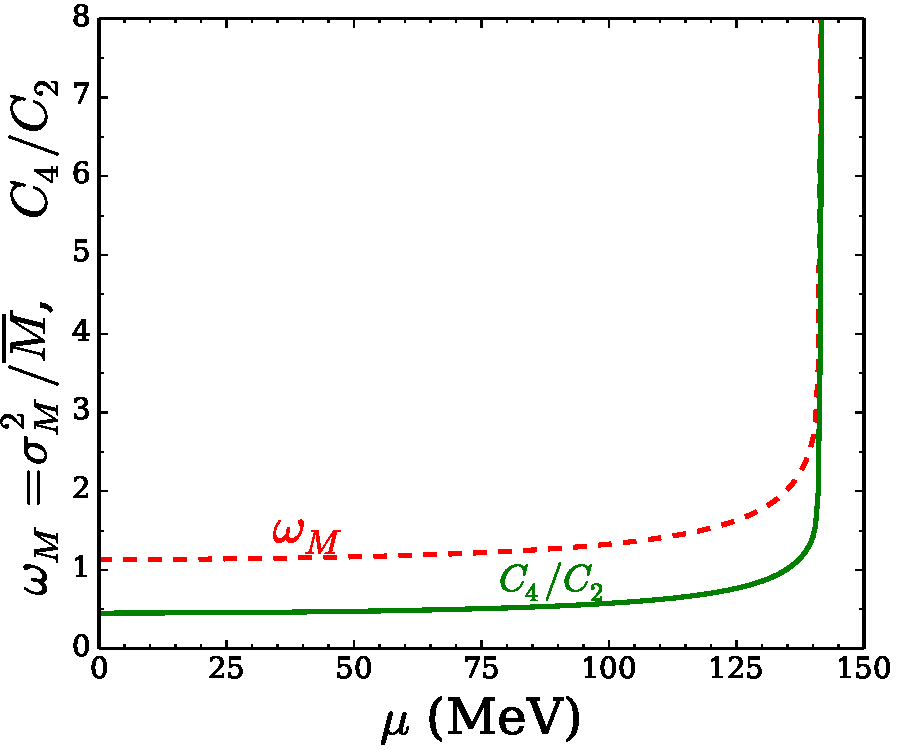
\includegraphics[width=0.4\textwidth]{figs/C4_bose}}
\caption{\label{fig:cheapbose}
Fluctuations for a canonical ensemble at fixed charge, $Q=0$, with an effective chemical potential, $\mu$, applied to adjust the net pion number in a volume of 500 fm$^3$ at a temperature of 100 MeV. The relative variance of the multiplicity distribution (dashed red line) and the ratio $C_4/C_2$ of the net-charge distribution (solid green line) grow dramatically as $\mu$ approaches the pion mass. Super-radiant effects can take place once $\mu$ reaches $m_\pi=139.57$ MeV. Heavy-ion collisions are expected to decouple with effective chemical potentials near 75 MeV, which is well below the onset of large fluctuations.
}
\end{figure}
As a function of the effective chemical potential $\mu$, the partition function for a pion gas in a volume of 500 fm$^3$ and at a temperature of 100 MeV was calculated from Eq. (\ref{eq:Zbf}). For $\mu$ in the range of of 75 MeV the relative variance of the charged multiplicity distribution is $\omega_M\approx 1.2$, which modestly increase $C_4/C_2$ as shown in Fig. \ref{fig:cheapbose} for a fixed efficiency of $\alpha=0.3$. More dramatic results for $C_4/C_2$ are not expected unless the chemical potential would get within a few MeV of the pion mass. As discussed above, this is not expected. However, if the number of pion sources fluctuated wildly from one event to another, and if there were some events with twice the number of sources emitting into the same phase space, super-radiance might occur in some small fraction of the events. Such behavior would strongly contradict expectations based on chemical equilibrium. 


\subsection{Hadron Gas}\label{sec:hadrongas_cheap}

Thus far, all the simple examples presented in this section considered a system with one type of conserved charge, whereas a hadron gas obeys the conservation of baryon number, strangeness and electric charge. This invalidates the use of the recurrence relation of Eq. (\ref{eq:savchuck}) and requires the application of Eq. (\ref{eq:recurrence}), or if Bose corrections are included, Eq. (\ref{eq:bose}). Here, we calculate the canonical ensemble, $Z_A(Q,B,S)$, using the recurrence relation, then apply the Monte Carlo techniques of Sec. \ref{sec:theoryMC} to generate sample sets of particles. The calculation is based on a large number, $\sim 300$, hadron resonances listed in \cite{Tanabashi:2018oca}. After generating the particles, unstable resonances are decayed. For this section, a uniform efficiency $\alpha$ is assumed, independent of species, momenta, or whether the products came from a weak decay (charged pions and kaons were not decayed).

Emission is assumed to come from sub-volumes, or patches, of fixed size. Because each volume is independent, there are no correlations between the various sub-volumes and because cumulants scale linearly with the number of sub-volumes, the ratios of cumulants depend only on the patch volume, not on the overall volume. However, if the number of patches fluctuates, the result would be modified by volume fluctuations. One would expect similar modifications as shown in Sec. \ref{sec:volumefluc}.

Here, the sensitivity to three parameters is investigated. The three parameters are the patch volume, the baryon density, and the fixed efficiency. When one parameter is varied, the other two are set at default values. The default calculation is that the temperature is set at $T=150$ MeV, the baryon density is set to $\rho_B=0$, the efficiency is $\alpha=0.3$ and the default patch volume is 200 fm$^3$. The net electric charge is set to by 0.4 times the average baryon density. After these sensitivities are studied, a calculation at finite baryon density is modified so that the net baryon charge responsible for the non-zero charge density is allowed to fluctuate according to a Poissonian distribution. This is motivated by the fact that the non-zero baryon density comes from charges transported far away from mid-rapidity at early times, so that local charge conservation should play little role for its distribution.

First, the dependence on patch size is exhibited in  Fig. \ref{fig:simple_patchsize}. For small patches the emission of baryons is discouraged because each baryon must be accompanied by the existence of an anti-baryon. Thus, the Boltzmann factor, $e^{-M/T}$, for the mass is compounded by the existence of a second....

% RACHEL -- make figures for
% Default T=150 MeV, Patch Volume=200 fm^3, alpha=0.3
% A. C_4/C_2 for net protons and for net charge with default+ rho_B=0 vs Volume
% B. C_4/C_2 for net protons and for net charge with default+ rho_B=0 vs alpha
% C. C_4/C_2 and C_3/C_1 for net protons and for net charge for default vs rho_B=0={0,0.02,0.04,0.06..., 0.3} with fixed charge
% D. Same as (C) but with "fixed" charge fluctuating according to Poisson about average
%


\section{Blast Wave Model with a Full Hadron Gas and Comparison to STAR Results}\label{sec:blast}



\section{Summary}\label{sec:summary}

\begin{acknowledgments}
This work was supported by the Department of Energy Office of Science through grant number DE-FG02-03ER41259 and through grant number DE-FG02-87ER40328. 
\end{acknowledgments}

\begin{thebibliography}{99}

%\cite{Schlichting:2010qia}
\bibitem{Schlichting:2010qia}
S.~Schlichting and S.~Pratt,
%``Charge conservation at energies available at the BNL Relativistic Heavy Ion Collider and contributions to local parity violation observables,''
Phys. Rev. C \textbf{83} (2011), 014913
doi:10.1103/PhysRevC.83.014913
[arXiv:1009.4283 [nucl-th]].
%149 citations counted in INSPIRE as of 19 May 2020

%\cite{Pratt:2010zn}
\bibitem{Pratt:2010zn}
S.~Pratt, S.~Schlichting and S.~Gavin,
%``Effects of Momentum Conservation and Flow on Angular Correlations at RHIC,''
Phys. Rev. C \textbf{84} (2011), 024909
doi:10.1103/PhysRevC.84.024909
[arXiv:1011.6053 [nucl-th]].
%95 citations counted in INSPIRE as of 19 May 2020

%\cite{Schlichting:2010na}
\bibitem{Schlichting:2010na}
S.~Schlichting and S.~Pratt,
%``Effects of Charge Conservation and Flow on Fluctuations of parity-odd Observables ar RHIC,''
[arXiv:1005.5341 [nucl-th]].
%28 citations counted in INSPIRE as of 19 May 2020

%\cite{Oliinychenko:2020cmr}
\bibitem{Oliinychenko:2020cmr}
D.~Oliinychenko, S.~Shi and V.~Koch,
%``Effects of local event-by-event conservation laws in ultra-relativistic heavy ion collisions at the particlization,''
[arXiv:2001.08176 [hep-ph]].
%0 citations counted in INSPIRE as of 19 May 2020

%\cite{Tanabashi:2018oca}
\bibitem{Tanabashi:2018oca}
M.~Tanabashi \textit{et al.} [Particle Data Group],
%``Review of Particle Physics,''
Phys. Rev. D \textbf{98} (2018) no.3, 030001
doi:10.1103/PhysRevD.98.030001
%4561 citations counted in INSPIRE as of 13 May 2020

%\cite{Savchuk:2019xfg}
\bibitem{Savchuk:2019xfg}
O.~Savchuk, R.~V.~Poberezhnyuk, V.~Vovchenko and M.~I.~Gorenstein,
%``Binomial acceptance corrections for particle number distributions in high-energy reactions,''
Phys. Rev. C \textbf{101} (2020) no.2, 024917
doi:10.1103/PhysRevC.101.024917
[arXiv:1911.03426 [hep-ph]].
%2 citations counted in INSPIRE as of 05 May 2020

%\cite{Oliinychenko:2020cmr}
\bibitem{Oliinychenko:2020cmr} 
  D.~Oliinychenko, S.~Shi and V.~Koch,
  %``Effects of local event-by-event conservation laws in ultra-relativistic heavy ion collisions at the particlization,''
  arXiv:2001.08176 [hep-ph].
  %%CITATION = ARXIV:2001.08176;%%
  
  %\cite{Pratt:1999ht}
\bibitem{Pratt:1999ht} 
  S.~Pratt and S.~Das Gupta,
  %``Statistical models of nuclear fragmentation,''
  Phys.\ Rev.\ C {\bf 62}, 044603 (2000)
  doi:10.1103/PhysRevC.62.044603
  [nucl-th/9903006].
  %%CITATION = doi:10.1103/PhysRevC.62.044603;%%
  %25 citations counted in INSPIRE as of 29 Mar 2020

%\cite{Cheng:2002jb}
\bibitem{Cheng:2002jb}
S.~Cheng and S.~Pratt,
%``Isospin fluctuations from a thermally equilibrated hadron gas,''
Phys.\ Rev.\ C \textbf{67}, 044904 (2003)
doi:10.1103/PhysRevC.67.044904
[arXiv:nucl-th/0207051 [nucl-th]].
%4 citations counted in INSPIRE as of 30 Mar 2020

\bibitem{Pratt:2003jd}
S.~Pratt and J.~Ruppert,
%``The Quark gluon plasma in a finite volume,''
Phys.\ Rev.\ C \textbf{68}, 024904 (2003)
doi:10.1103/PhysRevC.68.024904
[arXiv:nucl-th/0303043 [nucl-th]].
%6 citations counted in INSPIRE as of 30 Mar 2020

%\cite{Sangaline:2015bma}
\bibitem{Sangaline:2015bma}
E.~Sangaline,
%``Strongly Intensive Cumulants: Fluctuation Measures for Systems With Incompletely Constrained Volumes,''
[arXiv:1505.00261 [nucl-th]].
%15 citations counted in INSPIRE as of 20 May 2020

%\cite{Gorenstein:2011vq}
\bibitem{Gorenstein:2011vq}
M.~Gorenstein and M.~Gazdzicki,
%``Strongly Intensive Quantities,''
Phys. Rev. C \textbf{84} (2011), 014904
doi:10.1103/PhysRevC.84.014904
[arXiv:1101.4865 [nucl-th]].
%96 citations counted in INSPIRE as of 20 May 2020

%\cite{Gazdzicki:2013ana}
\bibitem{Gazdzicki:2013ana}
M.~Gazdzicki, M.~Gorenstein and M.~Mackowiak-Pawlowska,
%``Normalization of strongly intensive quantities,''
Phys. Rev. C \textbf{88} (2013) no.2, 024907
doi:10.1103/PhysRevC.88.024907
[arXiv:1303.0871 [nucl-th]].
%49 citations counted in INSPIRE as of 20 May 2020

%\cite{Begun:2014boa}
\bibitem{Begun:2014boa}
V.~V.~Begun, M.~I.~Gorenstein and K.~Grebieszkow,
%``Strongly Intensive Measures for Particle Number Fluctuations: Effects of Hadronic Resonances,''
J. Phys. G \textbf{42} (2015) no.7, 075101
doi:10.1088/0954-3899/42/7/075101
[arXiv:1409.3023 [nucl-th]].
%4 citations counted in INSPIRE as of 20 May 2020

%\cite{Greiner:1993jn}
\bibitem{Greiner:1993jn}
C.~Greiner, C.~Gong and B.~Muller,
%``Some remarks on pion condensation in relativistic heavy ion collisions,''
Phys. Lett. B \textbf{316} (1993), 226-230
doi:10.1016/0370-2693(93)90317-B
[arXiv:hep-ph/9307336 [hep-ph]].
%67 citations counted in INSPIRE as of 13 May 2020

%\cite{Pratt:1993uy}
\bibitem{Pratt:1993uy}
S.~Pratt,
%``Pion lasers from high-energy collisions,''
Phys. Lett. B \textbf{301} (1993), 159-164
doi:10.1016/0370-2693(93)90682-8
%136 citations counted in INSPIRE as of 13 May 2020

%\cite{Bzdak:2018uhv}
\bibitem{Bzdak:2018uhv}
A.~Bzdak, V.~Koch, D.~Oliinychenko and J.~Steinheimer,
%``Large proton cumulants from the superposition of ordinary multiplicity distributions,''
Phys. Rev. C \textbf{98} (2018) no.5, 054901
doi:10.1103/PhysRevC.98.054901
[arXiv:1804.04463 [nucl-th]].
%11 citations counted in INSPIRE as of 13 May 2020














%\cite{Pratt:2015zsa}
\bibitem{Pratt:2015zsa} 
  S.~Pratt, E.~Sangaline, P.~Sorensen and H.~Wang,
  %``Constraining the Eq. of State of Super-Hadronic Matter from Heavy-Ion Collisions,''
  Phys.\ Rev.\ Lett.\  {\bf 114}, 202301 (2015).
  %doi:10.1103/PhysRevLett.114.202301.
  %[arXiv:1501.04042 [nucl-th]].
  %%CITATION = doi:10.1103/PhysRevLett.114.202301;%%
  %62 citations counted in INSPIRE as of 21 Mar 2019
  
	
%\cite{Pratt:2015jsa}
\bibitem{Pratt:2015jsa} 
  S.~Pratt, W.~P.~McCormack and C.~Ratti,
  %``Production of Charge in Heavy Ion Collisions,''
  Phys.\ Rev.\ C {\bf 92}, 064905 (2015).
  %doi:10.1103/PhysRevC.92.064905
  %[arXiv:1508.07031 [nucl-th]].
  %%CITATION = doi:10.1103/PhysRevC.92.064905;%%
  %4 citations counted in INSPIRE as of 19 Dec 2017 
  
%\cite{Bernhard:2016tnd}
\bibitem{Bernhard:2016tnd} 
  J.~E.~Bernhard, J.~S.~Moreland, S.~A.~Bass, J.~Liu and U.~Heinz,
  %``Applying Bayesian parameter estimation to relativistic heavy-ion collisions: simultaneous characterization of the initial state and quark-gluon plasma medium,''
  Phys.\ Rev.\ C {\bf 94}, no. 2, 024907 (2016).
  %doi:10.1103/PhysRevC.94.024907
 % [arXiv:1605.03954 [nucl-th]].
  %%CITATION = doi:10.1103/PhysRevC.94.024907;%%
  %150 citations counted in INSPIRE as of 21 Mar 2019
  
%\cite{Bernhard:2015hxa}
\bibitem{Bernhard:2015hxa} 
  J.~E.~Bernhard, P.~W.~Marcy, C.~E.~Coleman-Smith, S.~Huzurbazar, R.~L.~Wolpert and S.~A.~Bass,
  %``Quantifying properties of hot and dense QCD matter through systematic model-to-data comparison,''
  Phys.\ Rev.\ C {\bf 91}, no. 5, 054910 (2015).
  %doi:10.1103/PhysRevC.91.054910
 % [arXiv:1502.00339 [nucl-th]].
  %%CITATION = doi:10.1103/PhysRevC.91.054910;%%
  %36 citations counted in INSPIRE as of 21 Mar 2019

%\cite{Burke:2013yra}
\bibitem{Burke:2013yra}
  K.~M.~Burke {\it et al.} [JET Collaboration],
  %``Extracting the jet transport coefficient from jet quenching in high-energy heavy-ion collisions,''
  Phys.\ Rev.\ C {\bf 90}, no. 1, 014909 (2014).
 % doi:10.1103/PhysRevC.90.014909
 % [arXiv:1312.5003 [nucl-th]].
  %%CITATION = doi:10.1103/PhysRevC.90.014909;%%
  %215 citations counted in INSPIRE as of 21 Mar 2019

%\cite{He:2018gks}
\bibitem{He:2018gks} 
  Y.~He, L.~G.~Pang and X.~N.~Wang,
  %``Bayesian extraction of jet energy loss distributions in heavy-ion collisions,''
  arXiv:1808.05310 [hep-ph].
  %%CITATION = ARXIV:1808.05310;%%
  %3 citations counted in INSPIRE as of 21 Mar 2019

%\cite{Xu:2017obm}
\bibitem{Xu:2017obm} 
  Y.~Xu, J.~E.~Bernhard, S.~A.~Bass, M.~Nahrgang and S.~Cao,
  %``Data-driven analysis for the temperature and momentum dependence of the heavy-quark diffusion coefficient in relativistic heavy-ion collisions,''
  Phys.\ Rev.\ C {\bf 97}, no. 1, 014907 (2018).
 % doi:10.1103/PhysRevC.97.014907
 % [arXiv:1710.00807 [nucl-th]].
  %%CITATION = doi:10.1103/PhysRevC.97.014907;%%
  %27 citations counted in INSPIRE as of 21 Mar 2019
  
\bibitem{Greif:2017byw} 
  M.~Greif, J.~A.~Fotakis, G.~S.~Denicol and C.~Greiner,
  Phys.\ Rev.\ Lett.\  {\bf 120}, 242301 (2018).

\bibitem{Pratt:2019fbj} 
  S.~Pratt,
  %``Calculating n-Point Charge Correlations in Evolving Systems,''
  arXiv:1908.01053 [nucl-th].

\bibitem{Borsanyi:2011sw}
  S.~Borsanyi, Z.~Fodor, S.~D.~Katz, S.~Krieg, C.~Ratti and K.~Szabo,
  %``Fluctuations of conserved charges at finite temperature from lattice QCD,''
  JHEP {\bf 1201}, 138 (2012).
 % [arXiv:1112.4416 [hep-lat]].
  %%CITATION = ARXIV:1112.4416;%%

%\cite{Aarts:2014nba}
\bibitem{Aarts:2014nba} 
  G.~Aarts, C.~Allton, A.~Amato, P.~Giudice, S.~Hands and J.~I.~Skullerud,
  %``Electrical conductivity and charge diffusion in thermal QCD from the lattice,''
  JHEP {\bf 1502}, 186 (2015).
  %doi:10.1007/JHEP02(2015)186
  %[arXiv:1412.6411 [hep-lat]].
  %%CITATION = doi:10.1007/JHEP02(2015)186;%%
  %71 citations counted in INSPIRE as of 27 Nov 2017

%\cite{Amato:2013naa}
\bibitem{Amato:2013naa} 
  A.~Amato, G.~Aarts, C.~Allton, P.~Giudice, S.~Hands and J.~I.~Skullerud,
  %``Electrical conductivity of the quark-gluon plasma across the deconfinement transition,''
  Phys.\ Rev.\ Lett.\  {\bf 111}, no. 17, 172001 (2013).
 % doi:10.1103/PhysRevLett.111.172001
 % [arXiv:1307.6763 [hep-lat]].
  %%CITATION = doi:10.1103/PhysRevLett.111.172001;%%
  %119 citations counted in INSPIRE as of 25 Mar 2019

%\cite{Policastro:2002se} diffusion from AdS-CFT
\bibitem{Policastro:2002se} 
  G.~Policastro, D.~T.~Son and A.~O.~Starinets,
  %``From AdS / CFT correspondence to hydrodynamics,''
  JHEP {\bf 0209}, 043 (2002).
 % doi:10.1088/1126-6708/2002/09/043
 % [hep-th/0205052].
  %%CITATION = doi:10.1088/1126-6708/2002/09/043;%%
  %641 citations counted in INSPIRE as of 25 Mar 2019

%\cite{CasalderreySolana:2006rq} D for heavy quarks from AdS/CFT
\bibitem{CasalderreySolana:2006rq} 
  J.~Casalderrey-Solana and D.~Teaney,
  %``Heavy quark diffusion in strongly coupled N=4 Yang-Mills,''
  Phys.\ Rev.\ D {\bf 74}, 085012 (2006).
  %doi:10.1103/PhysRevD.74.085012
  %[hep-ph/0605199].
  %%CITATION = doi:10.1103/PhysRevD.74.085012;%%
  %383 citations counted in INSPIRE as of 25 Mar 2019

%\cite{Ghiglieri:2018dib}
\bibitem{Ghiglieri:2018dib} 
  J.~Ghiglieri, G.~D.~Moore and D.~Teaney,
  %``QCD Shear Viscosity at (almost) NLO,''
  JHEP {\bf 1803}, 179 (2018).
  %doi:10.1007/JHEP03(2018)179
  %[arXiv:1802.09535 [hep-ph]].
  %%CITATION = doi:10.1007/JHEP03(2018)179;%%
  %13 citations counted in INSPIRE as of 01 May 2019
  
  
\bibitem{Greif:2016skc} 
  M.~Greif, C.~Greiner and G.~S.~Denicol,
  %``Electric conductivity of a hot hadron gas from a kinetic approach,''
  Phys.\ Rev.\ D {\bf 93}, no. 9, 096012 (2016)
  Erratum: [Phys.\ Rev.\ D {\bf 96}, no. 5, 059902 (2017)]
  
\bibitem{Hammelmann:2018ath} 
  J.~Hammelmann, J.~M.~Torres-Rincon, J.~B.~Rose, M.~Greif and H.~Elfner,
  %``Electrical conductivity and relaxation via colored noise in a hadronic gas,''
  Phys.\ Rev.\ D {\bf 99}, no. 7, 076015 (2019).

%\cite{Pratt:2018ebf}
\bibitem{Pratt:2018ebf} 
  S.~Pratt and C.~Plumberg,
  %``Evolving Charge Correlations in a Hybrid Model with both Hydrodynamics and Hadronic Boltzmann Descriptions,''
  to appear in Phys. Rev. C, arXiv:1812.05649 [nucl-th].
  %%CITATION = ARXIV:1812.05649;%%
  %1 citations counted in INSPIRE as of 11 Apr 2019

\bibitem{Shen:2014vra} 
  C.~Shen, Z.~Qiu, H.~Song, J.~Bernhard, S.~Bass and U.~Heinz,
  %``The iEBE-VISHNU code package for relativistic heavy-ion collisions,''
  Comput.\ Phys.\ Commun.\  {\bf 199}, 61 (2016)

%\cite{Pratt:2017oyf}
\bibitem{Pratt:2017oyf}
  S.~Pratt, J.~Kim and C.~Plumberg,
  %``Evolution of Charge Fluctuations and Correlations in the Hydrodynamic Stage of Heavy Ion Collisions,''
  Phys.\ Rev.\ C {\bf 98}, no. 1, 014904 (2018).
  %doi:10.1103/PhysRevC.98.014904.
%  [arXiv:1712.09298 [nucl-th]].
  %%CITATION = doi:10.1103/PhysRevC.98.014904;%%

%\cite{Wang:2012jua}
\bibitem{Wang:2012jua} %% Hui thesis
  H.~Wang, Ph.D. Thesis,
  %``Study of particle ratio fluctuations and charge balance functions at RHIC,''
  arXiv:1304.2073 [nucl-ex].
  %%CITATION = ARXIV:1304.2073;%%
  %4 citations counted in INSPIRE as of 29 Oct 2017

%\cite{Abelev:2010ab}
\bibitem{Abelev:2010ab} 
  B.~I.~Abelev {\it et al.} [STAR Collaboration],
  %``Longitudinal scaling property of the charge balance function in Au + Au collisions at 200 GeV,''
  Phys.\ Lett.\ B {\bf 690}, 239 (2010).
  %doi:10.1016/j.physletb.2010.05.028
  %[arXiv:1002.1641 [nucl-ex]].
  %%CITATION = doi:10.1016/j.physletb.2010.05.028;%%
  %10 citations counted in INSPIRE as of 14 Dec 2017

%\cite{Li:2011zzx}
%\bibitem{Li:2011zzx} 
  N.~Li {\it et al.} [STAR Collaboration],
  %``The study of longitudinal properties of the charge balance function,''
%  Indian J.\ Phys.\  {\bf 85}, 923 (2011).
  %doi:10.1007/s12648-011-0100-0
  %%CITATION = doi:10.1007/s12648-011-0100-0;%%

%\cite{Adams:2003kg}
\bibitem{Adams:2003kg} 
  J.~Adams {\it et al.} [STAR Collaboration],
  %``Narrowing of the balance function with centrality in au + au collisions at (S(NN))**1/2 = 130-GeV,''
  Phys.\ Rev.\ Lett.\  {\bf 90}, 172301 (2003).
  %doi:10.1103/PhysRevLett.90.172301
  %[nucl-ex/0301014].
  %%CITATION = doi:10.1103/PhysRevLett.90.172301;%%
  %88 citations counted in INSPIRE as of 14 Dec 2017 
   
%\cite{Aggarwal:2010ya}
\bibitem{Aggarwal:2010ya} 
  M.~M.~Aggarwal {\it et al.} [STAR Collaboration],
  %``Balance Functions from Au$+$Au, $d+$Au, and $p+p$ Collisions at $\sqrt{s_{NN}}$ = 200 GeV,''
  Phys.\ Rev.\ C {\bf 82}, 024905 (2010).
  %doi:10.1103/PhysRevC.82.024905
  %[arXiv:1005.2307 [nucl-ex]].
  %%CITATION = doi:10.1103/PhysRevC.82.024905;%%
  %43 citations counted in INSPIRE as of 14 Dec 2017

%\cite{Alt:2004gx}
%\bibitem{Alt:2004gx} 
 % C.~Alt {\it et al.} [NA49 Collaboration],
  %``System size and centrality dependence of the balance function in A + A collisions at s(NN)**(1/2) = 17.2-GeV,''
 % Phys.\ Rev.\ C {\bf 71}, 034903 (2005).
  %doi:10.1103/PhysRevC.71.034903
  %[hep-ex/0409031].
  %%CITATION = doi:10.1103/PhysRevC.71.034903;%%
  %36 citations counted in INSPIRE as of 14 Dec 2017

%\cite{Abelev:2013csa}
\bibitem{Abelev:2013csa}
  B.~Abelev {\it et al.} [ALICE Collaboration],
  %``Charge correlations using the balance function in Pb-Pb collisions at $\sqrt{s_{NN}}$ = 2.76 TeV,''
  Phys.\ Lett.\ B {\bf 723}, 267 (2013).
  %doi:10.1016/j.physletb.2013.05.039
  %[arXiv:1301.3756 [nucl-ex]].
  %%CITATION = doi:10.1016/j.physletb.2013.05.039;%%
  %22 citations counted in INSPIRE as of 14 Dec 2017
  %measured both for Delta phi and Delta eta
  
%\cite{Alt:2007hk}
\bibitem{Alt:2007hk} 
  C.~Alt {\it et al.} [NA49 Collaboration],
  %``Rapidity and energy dependence of the electric charge correlations in A + A collisions at the SPS energies,''
  Phys.\ Rev.\ C {\bf 76}, 024914 (2007).
  %doi:10.1103/PhysRevC.76.024914
  %[arXiv:0705.1122 [nucl-ex]].
  %%CITATION = doi:10.1103/PhysRevC.76.024914;%%
  %19 citations counted in INSPIRE as of 14 Dec 2017

%\cite{Adamczyk:2015yga}
\bibitem{Adamczyk:2015yga} 
  L.~Adamczyk {\it et al.} [STAR Collaboration],
  %``Beam-energy dependence of charge balance functions from Au + Au collisions at energies available at the BNL Relativistic Heavy Ion Collider,''
  Phys.\ Rev.\ C {\bf 94}, no. 2, 024909 (2016).
  %doi:10.1103/PhysRevC.94.024909
  %[arXiv:1507.03539 [nucl-ex]].
  %%CITATION = doi:10.1103/PhysRevC.94.024909;%%
  %3 citations counted in INSPIRE as of 29 Oct 2017

%\cite{Adamczyk:2013hsi}
\bibitem{Adamczyk:2013hsi} 
  L.~Adamczyk {\it et al.} [STAR Collaboration],
  %``Fluctuations of charge separation  perpendicular to the event plane and local parity violation in $\sqrt{s_{NN}}=200$ GeV Au+Au  collisions at the BNL Relativistic Heavy Ion Collider,''
  Phys.\ Rev.\ C {\bf 88}, no. 6, 064911 (2013).
 % doi:10.1103/PhysRevC.88.064911.
%  [arXiv:1302.3802 [nucl-ex]].
  %%CITATION = doi:10.1103/PhysRevC.88.064911;%%
  %57 citations counted in INSPIRE as of 20 Nov 2018

%\cite{Abelev:2009ac}
\bibitem{Abelev:2009ac} 
  B.~I.~Abelev {\it et al.} [STAR Collaboration],
  %``Azimuthal Charged-Particle Correlations and Possible Local Strong Parity Violation,''
  Phys.\ Rev.\ Lett.\  {\bf 103}, 251601 (2009).
 % doi:10.1103/PhysRevLett.103.251601.
%  [arXiv:0909.1739 [nucl-ex]].
  %%CITATION = doi:10.1103/PhysRevLett.103.251601;%%
  %397 citations counted in INSPIRE as of 20 Nov 2018

\bibitem{Bass:2000az} 
  S.~A.~Bass, P.~Danielewicz and S.~Pratt,
  %``Clocking hadronization in relativistic heavy ion collisions with balance functions,''
  Phys.\ Rev.\ Lett.\  {\bf 85}, 2689 (2000).

%\cite{Pratt:2012dz}
\bibitem{Pratt:2012dz} 
  S.~Pratt,
  %``Identifying the Charge Carriers of the Quark-Gluon Plasma,''
  Phys.\ Rev.\ Lett.\  {\bf 108}, 212301 (2012).
  %doi:10.1103/PhysRevLett.108.212301
  %[arXiv:1203.4578 [nucl-th]].
  %%CITATION = doi:10.1103/PhysRevLett.108.212301;%%
  %22 citations counted in INSPIRE as of 19 Dec 2017


%\cite{Pan:2014caa}
\bibitem{Pan:2014caa} 
  Y.~Pan and S.~Pratt,
  %``Baryon annihilation and regeneration in heavy ion collisions,''
  Phys.\ Rev.\ C {\bf 89}, no. 4, 044911 (2014).
  %doi:10.1103/PhysRevC.89.044911
  %%CITATION = doi:10.1103/PhysRevC.89.044911;%%
  %10 citations counted in INSPIRE as of 19 Dec 2017

%\cite{Steinheimer:2017vju}
\bibitem{Steinheimer:2017vju} 
  J.~Steinheimer, J.~Aichelin, M.~Bleicher and H.~Stöcker,
  %``Influence of the hadronic phase on observables in ultrarelativistic heavy ion collisions,''
  Phys.\ Rev.\ C {\bf 95}, no. 6, 064902 (2017).
  %doi:10.1103/PhysRevC.95.064902
  %[arXiv:1703.06638 [nucl-th]].
  %%CITATION = doi:10.1103/PhysRevC.95.064902;%%
  %5 citations counted in INSPIRE as of 19 Dec 2017
 
%\cite{Steinheimer:2012rd}
\bibitem{Steinheimer:2012rd} 
  J.~Steinheimer, J.~Aichelin and M.~Bleicher,
  %``Nonthermal p/? Ratio at LHC as a Consequence of Hadronic Final State Interactions,''
  Phys.\ Rev.\ Lett.\  {\bf 110}, no. 4, 042501 (2013).
  %doi:10.1103/PhysRevLett.110.042501
  %[arXiv:1203.5302 [nucl-th]].
  %%CITATION = doi:10.1103/PhysRevLett.110.042501;%%
  %84 citations counted in INSPIRE as of 19 Dec 2017
  
%%%%%%%%%%%%%%%%%%%%%%% XXXXXXX

\begin{comment}

%\cite{Bellwied:2015lba}
%\bibitem{Bellwied:2015lba} 
  R.~Bellwied, S.~Borsanyi, Z.~Fodor, S.~D.~Katz, A.~Pasztor, C.~Ratti and K.~K.~Szabo,
  %``Fluctuations and correlations in high temperature QCD,''
  Phys.\ Rev.\ D {\bf 92}, no. 11, 114505 (2015).
 % doi:10.1103/PhysRevD.92.114505.
%  [arXiv:1507.04627 [hep-lat]].
  %%CITATION = doi:10.1103/PhysRevD.92.114505;%%
  %74 citations counted in INSPIRE as of 28 Mar 2018


%\bibitem{Ling:2013ksb} 
  B.~Ling, T.~Springer and M.~Stephanov,
  %``Hydrodynamics of charge fluctuations and balance functions,''
  Phys.\ Rev.\ C {\bf 89}, no. 6, 064901 (2014).

%\cite{Bozek:2004dt}
%\bibitem{Bozek:2004dt} 
  P.~Bozek,
  %``The Balance functions in azimuthal angle is a measure of the transverse flow,''
  Phys.\ Lett.\ B {\bf 609}, 247 (2005).
  %doi:10.1016/j.physletb.2005.01.072
  %[nucl-th/0412076].
  %%CITATION = doi:10.1016/j.physletb.2005.01.072;%%
  %29 citations counted in INSPIRE as of 19 Dec 2017


%\cite{Cheng:2004zy}
%\bibitem{Cheng:2004zy} 
  S.~Cheng, S.~Petriconi, S.~Pratt, M.~Skoby, C.~Gale, S.~Jeon, V.~Topor Pop and Q.~H.~Zhang,
  %``Statistical and dynamic models of charge balance functions,''
  Phys.\ Rev.\ C {\bf 69}, 054906 (2004).
  %doi:10.1103/PhysRevC.69.054906
  %[nucl-th/0401008].
  %%CITATION = doi:10.1103/PhysRevC.69.054906;%%
  %35 citations counted in INSPIRE as of 19 Dec 2017

%\bibitem{popcorn}
	P. Ed\'en and G. Gustafson, Zeit. f\"ur Phys. C, {\bf 75}, 41 (1997).

%\bibitem{urqmd}
	S.A.Bass et al [URQMD], Progr. Part. Nucl. Physics Vol. \textbf{41}, 225 (1998).

%\cite{Alt:2007hk}
%\bibitem{Alt:2007hk} 
  C.~Alt {\it et al.} [NA49 Collaboration],
  %``Rapidity and energy dependence of the electric charge correlations in A + A collisions at the SPS energies,''
  Phys.\ Rev.\ C {\bf 76}, 024914 (2007).
  %doi:10.1103/PhysRevC.76.024914
  %[arXiv:0705.1122 [nucl-ex]].
  %%CITATION = doi:10.1103/PhysRevC.76.024914;%%
  %19 citations counted in INSPIRE as of 14 Dec 2017

%\cite{Adamczyk:2015yga}
%\bibitem{Adamczyk:2015yga} 
  L.~Adamczyk {\it et al.} [STAR Collaboration],
  %``Beam-energy dependence of charge balance functions from Au + Au collisions at energies available at the BNL Relativistic Heavy Ion Collider,''
  Phys.\ Rev.\ C {\bf 94}, no. 2, 024909 (2016).
  %doi:10.1103/PhysRevC.94.024909
  %[arXiv:1507.03539 [nucl-ex]].
  %%CITATION = doi:10.1103/PhysRevC.94.024909;%%
  %3 citations counted in INSPIRE as of 29 Oct 2017

%\cite{Pan:2015pzh}
%\bibitem{Pan:2015pzh} 
  Y.~H.~Pan and W.~N.~Zhang,
  %``Charge balance functions in a scenario of continuing charge production in quark matter,''
  Eur.\ Phys.\ J.\ A {\bf 51}, no. 11, 147 (2015).
  %doi:10.1140/epja/i2015-15147-3
  %%CITATION = doi:10.1140/epja/i2015-15147-3;%%

%\bibitem{Heinz:2013wva} 
  U.~W.~Heinz,
  %``Towards the Little Bang Standard Model,''
  J.\ Phys.\ Conf.\ Ser.\  {\bf 455}, 012044 (2013).

%\bibitem{sorgepionwind}
	H. Sorge, Phys. Lett. B 373, 16 􏰞1993􏰀.
	
%\cite{Pratt:1998gt}
%\bibitem{Pratt:1998gt} 
  S.~Pratt and J.~Murray,
  %``Modeling the breakup stage of relativistic heavy ion collisions,''
  Phys.\ Rev.\ C {\bf 57}, 1907 (1998).
  %doi:10.1103/PhysRevC.57.1907
  %%CITATION = doi:10.1103/PhysRevC.57.1907;%%
  %23 citations counted in INSPIRE as of 27 Nov 2018
 

%\cite{Novak:2013bqa}
%\bibitem{Novak:2013bqa} 
  J.~Novak, K.~Novak, S.~Pratt, J.~Vredevoogd, C.~Coleman-Smith and R.~Wolpert,
  %``Determining Fundamental Properties of Matter Created in Ultrarelativistic Heavy-Ion Collisions,''
  Phys.\ Rev.\ C {\bf 89}, no. 3, 034917 (2014).
 % doi:10.1103/PhysRevC.89.034917.
 % [arXiv:1303.5769 [nucl-th]].
  %%CITATION = doi:10.1103/PhysRevC.89.034917;%%
  %61 citations counted in INSPIRE as of 29 Nov 2018 




%\cite{Shen:2014vra}
%\bibitem{Shen:2014vra} 
  C.~Shen, Z.~Qiu, H.~Song, J.~Bernhard, S.~Bass and U.~Heinz,
  %``The iEBE-VISHNU code package for relativistic heavy-ion collisions,''
  Comput.\ Phys.\ Commun.\  {\bf 199}, 61 (2016).

%\bibitem{Huovinen:2009yb} 
  P.~Huovinen and P.~Petreczky,
  %``QCD Equation of State and Hadron Resonance Gas,''
  Nucl.\ Phys.\ A {\bf 837}, 26 (2010).

%\bibitem{Kapusta:2014dja} 
  J.~I.~Kapusta and C.~Young,
  %``Causal Baryon Diffusion and Colored Noise,''
  Phys.\ Rev.\ C {\bf 90}, no. 4, 044902 (2014).

%\cite{Kapusta:2017hfi}
%\bibitem{Kapusta:2017hfi} 
  J.~I.~Kapusta and C.~Plumberg,
  %``Causal Electric Charge Diffusion and Balance Functions in Relativistic Heavy Ion Collisions,''
  Phys.\ Rev.\ C {\bf 97}, no. 1, 014906 (2018).
 % doi:10.1103/PhysRevC.97.014906.
 % [arXiv:1710.03329 [nucl-th]].
  %%CITATION = doi:10.1103/PhysRevC.97.014906;%%
  %8 citations counted in INSPIRE as of 13 Dec 2018
  
%\cite{Aziz:2004qu}
%\bibitem{Aziz:2004qu} 
  M.~A.~Aziz and S.~Gavin,
  %``Causal diffusion and the survival of charge fluctuations in nuclear collisions,''
  Phys.\ Rev.\ C {\bf 70}, 034905 (2004).
%  doi:10.1103/PhysRevC.70.034905.
 % [nucl-th/0404058].
  %%CITATION = doi:10.1103/PhysRevC.70.034905;%%
  %58 citations counted in INSPIRE as of 28 Nov 2018

%\bibitem{Cooper:1974mv} 
  F.~Cooper and G.~Frye,
  %``Comment on the Single Particle Distribution in the Hydrodynamic and Statistical Thermodynamic Models of Multiparticle Production,''
  Phys.\ Rev.\ D {\bf 10}, 186 (1974).

%\bibitem{Huovinen:2012is} 
  P.~Huovinen and H.~Petersen,
  %``Particlization in hybrid models,''
  Eur.\ Phys.\ J.\ A {\bf 48}, 171 (2012).

%\cite{Becattini:2012sq}
%\bibitem{Becattini:2012sq} 
  F.~Becattini, M.~Bleicher, T.~Kollegger, M.~Mitrovski, T.~Schuster and R.~Stock,
  %``Hadronization and Hadronic Freeze-Out in Relativistic Nuclear Collisions,''
  Phys.\ Rev.\ C {\bf 85}, 044921 (2012).
  %doi:10.1103/PhysRevC.85.044921
  %[arXiv:1201.6349 [nucl-th]].
  %%CITATION = doi:10.1103/PhysRevC.85.044921;%%
  %59 citations counted in INSPIRE as of 19 Dec 2017

%\cite{Becattini:2012xb}
%\bibitem{Becattini:2012xb} 
  F.~Becattini, M.~Bleicher, T.~Kollegger, T.~Schuster, J.~Steinheimer and R.~Stock,
  %``Hadron Formation in Relativistic Nuclear Collisions and the QCD Phase Diagram,''
  Phys.\ Rev.\ Lett.\  {\bf 111}, 082302 (2013).
  %doi:10.1103/PhysRevLett.111.082302
  %[arXiv:1212.2431 [nucl-th]].
  %%CITATION = doi:10.1103/PhysRevLett.111.082302;%%
  %110 citations counted in INSPIRE as of 19 Dec 2017

%\cite{Pratt:2014vja}
%\bibitem{Pratt:2014vja} 
  S.~Pratt,
  %``Accounting for backflow in hydrodynamic-Boltzmann interfaces,''
  Phys.\ Rev.\ C {\bf 89}, no. 2, 024910 (2014).
  %doi:10.1103/PhysRevC.89.024910
  %[arXiv:1401.0316 [nucl-th]]
  %%CITATION = doi:10.1103/PhysRevC.89.024910;%%
  %8 citations counted in INSPIRE as of 19 Dec 2017
%
%\bibitem{Pratt:2010jt} 
  S.~Pratt and G.~Torrieri,
  %``Coupling Relativistic Viscous Hydrodynamics to Boltzmann Descriptions,''
  Phys.\ Rev.\ C {\bf 82}, 044901 (2010).

%\cite{Bozek:2003qi}
%\bibitem{Bozek:2003qi} 
  P.~Bozek, W.~Broniowski and W.~Florkowski,
  %``Balance functions in a thermal model with resonances,''
  Acta Phys.\ Hung.\ A {\bf 22}, 149 (2005).
  %doi:10.1556/APH.22.2005.1-2.15
  %[nucl-th/0310062].
  %%CITATION = doi:10.1556/APH.22.2005.1-2.15;%%
  %35 citations counted in INSPIRE as of 19 Dec 2017

%\bibitem{WestfallAcceptance}
% Routines for modeling the efficiency of the STAR detector were generously provided by Gary Westfall.

%\cite{Steinheimer:2012bn}
%\bibitem{Steinheimer:2012bn} 
  J.~Steinheimer, V.~Koch and M.~Bleicher,
  %``Hydrodynamics at large baryon densities: Understanding proton vs. anti-proton v_2 and other puzzles,''
  Phys.\ Rev.\ C {\bf 86}, 044903 (2012).
  %doi:10.1103/PhysRevC.86.044903
  %[arXiv:1207.2791 [nucl-th]].
  %%CITATION = doi:10.1103/PhysRevC.86.044903;%%
  %36 citations counted in INSPIRE as of 19 Dec 2017

%\cite{Pratt:2003gh}
%\bibitem{Pratt:2003gh} 
  S.~Pratt and S.~Cheng,
  %``Removing distortions from charge balance functions,''
  Phys.\ Rev.\ C {\bf 68}, 014907 (2003).
  %doi:10.1103/PhysRevC.68.014907.
  %[nucl-th/0303025].
  %%CITATION = doi:10.1103/PhysRevC.68.014907;%%
  %28 citations counted in INSPIRE as of 29 Nov 2018
 
%\cite{Schlichting:2010qia}
%\bibitem{Schlichting:2010qia} 
  S.~Schlichting and S.~Pratt,
  %``Charge conservation at energies available at the BNL Relativistic Heavy Ion Collider and contributions to local parity violation observables,''
  Phys.\ Rev.\ C {\bf 83}, 014913 (2011).
 % doi:10.1103/PhysRevC.83.014913.
 % [arXiv:1009.4283 [nucl-th]].
  %%CITATION = doi:10.1103/PhysRevC.83.014913;%%
  %120 citations counted in INSPIRE as of 30 Nov 2018

%\cite{Pratt:2010zn}
%\bibitem{Pratt:2010zn} 
  S.~Pratt, S.~Schlichting and S.~Gavin,
  %``Effects of Momentum Conservation and Flow on Angular Correlations at RHIC,''
  Phys.\ Rev.\ C {\bf 84}, 024909 (2011).
  %doi:10.1103/PhysRevC.84.024909.
  %[arXiv:1011.6053 [nucl-th]].
  %%CITATION = doi:10.1103/PhysRevC.84.024909;%%
  %74 citations counted in INSPIRE as of 30 Nov 2018  

%\bibitem{Gelis:2013rba} 
  T.~Epelbaum and F.~Gelis,
  %``Pressure isotropization in high energy heavy ion collisions,''
  Phys.\ Rev.\ Lett.\  {\bf 111}, 232301 (2013).

%\bibitem{Dusling:2010rm} 
  K.~Dusling, T.~Epelbaum, F.~Gelis and R.~Venugopalan,
  %``Role of quantum fluctuations in a system with strong fields: Onset of hydrodynamical flow,''
  Nucl.\ Phys.\ A {\bf 850}, 69 (2011).

%\bibitem{Vredevoogd:2008id} 
  J.~Vredevoogd and S.~Pratt,
  %``Universal Flow in the First Stage of Relativistic Heavy Ion Collisions,''
  Phys.\ Rev.\ C {\bf 79}, 044915 (2009).
 % doi:10.1103/PhysRevC.79.044915.
 % [arXiv:0810.4325 [nucl-th]].
  %%CITATION = doi:10.1103/PhysRevC.79.044915;%%
  %80 citations counted in INSPIRE as of 02 Dec 2018

\end{comment}
         
\end{thebibliography}

\end{document}
